\subsubsubsubsection{Crossroads config reader}
\begin{figure}[h]
\centering
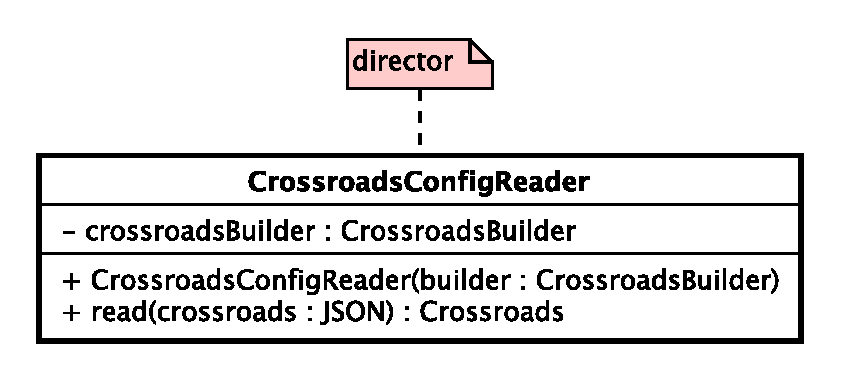
\includegraphics[scale=0.6,keepaspectratio]{images/solution/app/backend/crossroads_config_reader.eps}
\caption{\pReactiveBuild::CrossroadsConfigReader}
\label{fig:sd-app-crossroads-config-reader}
\end{figure}
\FloatBarrier
\begin{itemize}
  \item \textbf{\descr} \\
    It represents the concrete director of the crossroads builder.
    It has the responsibility to parse serializations of crossroads.
    \item \textbf{\attrs}
  \begin{itemize}
    \item \texttt{builder: CrossroadsBuilder} \\
The builder object which builds parts of the district.
  \end{itemize}
  \item \textbf{\ops}
  \begin{itemize} 
    \item[+] \texttt{CrossroadsConfigReader(builder: CrossroadsBuilder)} \\
Creates a concrete crossroads director with its own crossroads builder.
    \item[+] \texttt{read(crossroads: JSON) : Crossroads} \\
Parses a serialization of a crossroads.
It uses the builder multiple times 
to create incrementally a configuration of the requested crossroads as specified
in the configuration file. 
  \end{itemize}
\end{itemize}
